\section{ОХОРОНА ПРАЦІ}
\subsection{Значення охорони праці для забезпечення безпечних і здорових умов праці}
\par Значення охорони праці в будь-якій галузі України є дуже вагоме, адже саме охорона праці напряму пов'язана з вивченням та вирішенням питань безпеки праці на виробництві, попередженні виробничого травматизму і професійних захворювань, пожеж та вибухів, а також охорони навколишнього середовища.
\par При проведенні робіт нерідко порушуються діючі правила й інструкції з техніки безпеки. Це відбувається по причині незадовільного інструктажу й навчання робітників,  внаслідок неправильної організації робіт, недостатнього технічного нагляду зі сторони інженерно-технічних працівників.
\par Охорона праці та навколишнього середовища здійснюється на основі правових норм України і розглядає основи наукової організації праці робітників системи буріння нафтових і газових свердловин, питання виробничої санітарії, основи електробезпеки і техніки безпеки при монтажі і експлуатації бурового обладнання, моніторингу за роботою електороустановок на бурових, збором інформації з вимірювальних приладів бурових, що є важливим. 
\par Для того щоб максимально знизити травматизм, необхідна висока кваліфікація робітників, знання технологічних особливостей процесу буріння свердловин, призначення, конструкції та правила експлуатації устаткування й механізмів, правильних й безпечних прийомів виконання робіт, а також високий рівень технічного нагляду зі сторони керівників робіт.
\par Покращення організації праці, механізації тяжких й трудомістких робіт, раціоналізація технологічних процесів, впровадження нових, більш сучасних видів устаткування, механізмів та інструменту — основний напрям  підвищення продуктивності праці й створення здорової і безпечної виробничої обстановки на бурових підприємствах.

\subsection{Аналіз потенційних небезпек та шкідливих факторів виробничого середовища}

\par Важливою умовою функціонування будь-якого сучасного підриємства є робота із ЕОМ(електронно-обчислювальними машинами). Проте ця робота супроводжується впливом багатьох чиннів на організм оператора по роботі з ЕОМ. Було проведено аналіз і зроблено характеристику несприятливих виробничих факторів, які здатні впливати на здоров'я та самопочуття працівника. Всі дані наведено в таблиці \ref{t:safety1}.

{\footnotesize
\begin{longtable}{|p{4cm}|p{12cm}|}
\captionsetup{justification=centering}
\caption{Аналіз потенційних небезпек виробничих факторів при роботі з ЕОМ}\label{t:safety1}\\
\hline
\multicolumn{1}{|c|}{\textbf{Джерело небезпек}}&
\multicolumn{1}{p{12cm}|}{\textbf{Характеристика потенційно-небезпечних виробничих факторів та їх допустимі значення}}\\\hline

\endfirsthead
\caption*{\hfill Продовження таблиці \ref{t:safety1}}\\\hline

\multicolumn{1}{|c|}{\textbf{Джерело небезпек}}&
\multicolumn{1}{p{12cm}|}{\textbf{Характеристика потенційно-небезпечних виробничих факторів та їх допустимі значення}}\\\hline
\endhead

ренгенівське випромінювання	& Фактичні (середні) дані вимірів 9-12мкР/год (в діапазоні 1.2КеВ). Гранично допустима експозиційна доза: 1000мкР/год.  	\\ \hline


ультрафіолетове випромінювання & Фактичні дані вимірів: 0.001 Вт/м$^2$ в діапазоні 280-315 нм - УФ-Ф). Допустима інтенсивність: 0.01 Вт$^2$ -- УФ-В\\ \hline


ІЧ-випромінювання 	& 	Фактичні дані вимірів інтенсивності теплового випромінювання 0,05-4 Вт/м$^2$ (в діапазоні 700 нм-1мм). Допустима інтенсивність:  35-70 Вт/м$^2$.	\\ \hline

видимий діапазон  	& 	Фактичні дані: 0,1-2 Вт/м$^2$ (в діапазоні 320-400 нм) і 2,5-4 Вт/м$^2$ (в діапазоні 400-700 нм). Допустима інтенсивність потоку енергії:  10 Вт/м$^2$.	\\ \hline


яскравість 	& 	Фактичні дані: 306 кд/м$^2$. Допустиме значення: 35 кд/м$^2$.	\\ \hline

електростатичне поле & Фактичні дані: 15 кВ/м (0 Гц) Допустима напруженість поля  20-60 кВ/м.\\ \hline

шум 	& 	Діюче значення звукового тиску: 28.6-44 дБА. Допустиме значення: 55дБА
	\\ \hline

\end{longtable}
}

\par Робота оператора з ЕОМ вимагає максимальної концентрації протягом цілого робочого дня, що в свою чергу призводить до значних навантажень на організм. Також через постійне розумове навантаження зростає ризик перевантаження аналізаторів та ймовірність психічного розладу.



\subsection{Забезпечення нормальних умов праці при роботі з ЕОМ}
\par Для забезпечення нормальних умов праці оператора з ЕОМ потрібно створити максимально комфортні умови праці. Для цього було обрано робочий кабінет, який відповідає всім вимогах та стандартам праці.
\par В робочому кабінеті будуть знаходитися 11 робочих місць (рисунок \ref{pic:safety_room}). На кожного працівника розраховано одна одиниця техніки (сюди входить монітор, системний блок, клавіатура, мишка). Проте деякі працівники, у зв'язку зі специфічним видом роботи, потребуються два монітори, які розташовані поряд один з один. Кожний працівник відгороджений від інших дерев'яною перегородкою. Кожний працівник забезпечений робочим місцем загальною площею 8м$^2$. 

\begin{figure}[!ht]
\centering
		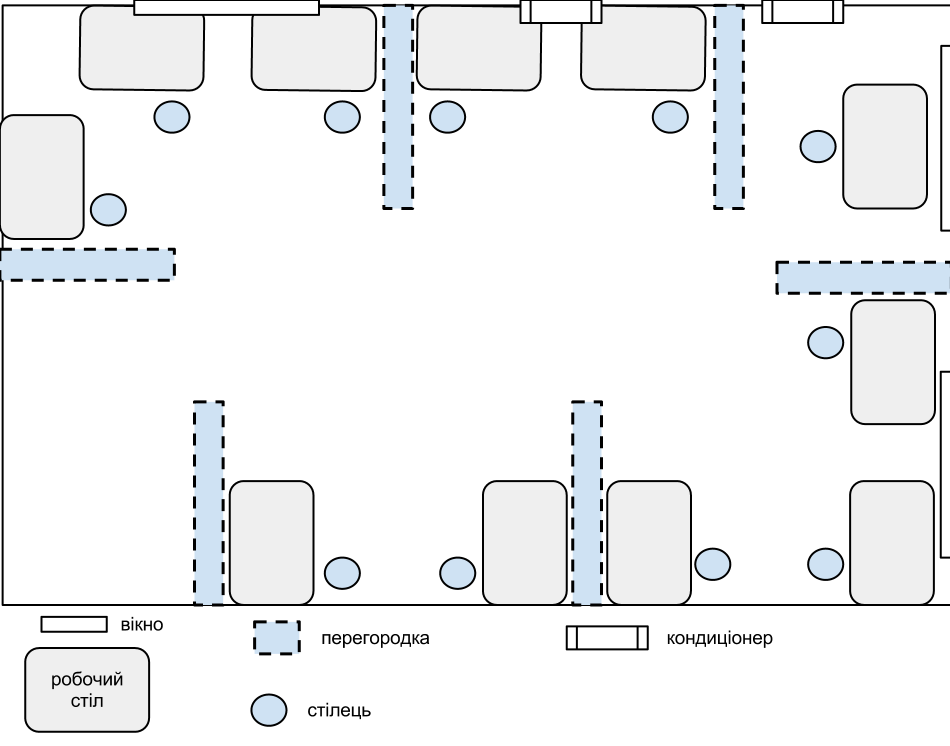
\includegraphics[width=1\textwidth]{safety_room.png}
		\captionof{figure}{Схема робочої кімнати - офісу}\label{pic:safety_room}
\end{figure}

\par Також для кожного працівника, для того щоб забезпечити комфортні умови праці розраховано три висувні ящики та тумбочку для власних речей, та шафки зверху робочого місця, для швидкого доступу до документації та канцелярських речей, що в свою чергу становить загальний об'ємом 22м$^2$. Кожний працівник забезпечується зручним та комфортним кріслом, яке регулюється згідно вимог. Все це зроблено із урахуванням ГОСТ 12.2.032-78, ДНАОП 0.00-1.31-99 та ДСан ПіН 3.3.2.007-98.



\par На кожному вікні є жалюзі, що дає змогу зменшити вплив сонячних променів на працюючого (засліплення монітору для прикладу).
\par Комп'ютерна-та електромережа прокладена із врахуванням всіх вимог техніки безпеки.
\par Крім обчислювальних одиниць, більше технічних засобів в кімнаті не передбачається, адже всі переферійні пристрої розташовані на коридорі.

\par Для забезпечення мікрокліматичних умов праці передбачено два кондиціонери, які можуть працювати в автоматичному режимі і підтримувати сталу температуру приміщення. Також налагоджено роботу постійної вентиляція , яка працює за наступним принципом: вентиляційні витяжки розміщені в 4 місцях (по кутах) кімнати. Дві із них працюють як витяжки, тобто втягують повітря, інші дві забезпечують свіжим повітрям кімнату -- в кінцевому результаті постійна циркуляція повітря. Вентиляційні труби виведені на вулицю. В таблиці \ref{t:safety_microclimate} наведено оптимальні значення метеорологічних умов в робочому кабінеті для легкої категорії робіт.


{\footnotesize
\begin{longtable}{|c|c|c|c|}
\captionsetup{justification=centering}
\caption{Оптимальні значення метеорологічних умов в робочому кабінеті для легкої категорії робіт}\label{t:safety_microclimate}\\
\hline
\multicolumn{1}{|c|}{\textbf{Період року}}&
\multicolumn{1}{c|}{\textbf{Температура, $^{\circ}$C}}&
\multicolumn{1}{c|}{\textbf{Відносна вологість, \%}}&
\multicolumn{1}{c|}{\textbf{Швидкість руху повітря, м/с}}\\ \hline

\endfirsthead
\caption*{\hfill Продовження таблиці \ref{t:safety_microclimate}}\\ \hline

\multicolumn{1}{|c|}{\textbf{Період року}}&
\multicolumn{1}{c|}{\textbf{Температура, $^{\circ}$C}}&
\multicolumn{1}{c|}{\textbf{Відносна вологість, \%}}&
\multicolumn{1}{c|}{\textbf{Швидкість руху повітря, м/с}}\\ \hline
\endhead
Теплий & 24-25 & 50-65 & 0.1-0.4 \\ \hline
\end{longtable}
}

\par Як згадувалося вище про вентиляцію -- саме вентиляція є основою забезпечення комфортних умов праці, тобто регуляцію мікроклімату. Характеристику штучної вентиляції наведено в таблиці \ref{t:safety_ventil}

{\footnotesize
\begin{longtable}{|c|c|c|c|}
\captionsetup{justification=centering}
\caption{Оптимальні значення метеорологічних умов в робочому кабінеті для легкої категорії робіт}\label{t:safety_ventil}\\
\hline
\multicolumn{1}{|c|}{\textbf{Приміщення}}&
\multicolumn{1}{c|}{\textbf{Тип вентиляції}}&
\multicolumn{1}{c|}{\textbf{Вентиляційне обладнання}}&
\multicolumn{1}{p{3cm}|}{\textbf{Кратність повітряного обміну, 1/год }}\\ \hline

\endfirsthead
\caption*{\hfill Продовження таблиці \ref{t:safety_ventil}}\\ \hline

\multicolumn{1}{|c|}{\textbf{Приміщення}}&
\multicolumn{1}{c|}{\textbf{Тип вентиляції}}&
\multicolumn{1}{c|}{\textbf{Вентиляційне обладнання}}&
\multicolumn{1}{p{3cm}|}{\textbf{Кратність повітробміну, 1/год }}\\ \hline
\endhead
Офіс & Механічна & Кондиціонер (700-1000 м$^3$/год, 4 кВт) & 2.2 \\ \hline
\end{longtable}
}

\par Так як робота людини з ЕОМ більше як на 90\% складається із зорової роботи -- тому правильне і раціональне освітлення становить основу для створення сприятливих умов праці та унеможливлення розвитку професійних захворювань. Освітлення повинне забезпечувати комфортну роботу працівника в будь-яку пору дня, чи то ранок, чи обід чи вечір. Характеристика штучної освітленості робочих місць
наводиться у таблиці \ref{t:safety_shtychno}

{\footnotesize
\begin{longtable}{|c|c|c|c|c|c|}
\captionsetup{justification=centering}
\caption{Оптимальні значення метеорологічних умов в робочому кабінеті для легкої категорії робіт}\label{t:safety_shtychno}\\
\hline
\multicolumn{1}{|c|}{\textbf{Приміщення}}&
\multicolumn{1}{p{2cm}|}{\textbf{Розряд зорової роботи}}&
\multicolumn{1}{p{2cm}|}{\textbf{Загальне освітлення, лК}}&
\multicolumn{1}{p{2.5cm}|}{\textbf{Комбіноване освітлення, лК}}&
\multicolumn{1}{p{3cm}|}{\textbf{Аварійне освітлення для продовження роботи, лК}}&
\multicolumn{1}{p{2.5cm}|}{\textbf{Аварійне освітлення для евакуації, лК}}\\ \hline

 \hline

\endfirsthead
\caption*{\hfill Продовження таблиці \ref{t:safety_shtychno}}\\ \hline

\multicolumn{1}{|c|}{\textbf{Приміщення}}&
\multicolumn{1}{p{2cm}|}{\textbf{Розряд зорової роботи}}&
\multicolumn{1}{p{2cm}|}{\textbf{Загальне освітлення, лК}}&
\multicolumn{1}{p{2.5cm}|}{\textbf{Комбіноване освітлення, лК}}&
\multicolumn{1}{p{3cm}|}{\textbf{Аварійне освітлення для продовження роботи, лК}}&
\multicolumn{1}{p{2.5cm}|}{\textbf{Аварійне освітлення для евакуації, лК}}\\ \hline
\endhead
Офіс & IV & 150-300 & 300-750 & 100-200 & 50-200\\ \hline
\end{longtable}
}

\par Засоби індивідуального захисту не передбачаються, так як монітори побудовані на основі рідких кристалів, тому тут немає регенерації картинки, потім завжди сталий.



\subsection{Забезпечення безпеки монтажу, пусконалагоджувальних, ремонтних робіт та експлуатації ЕОМ і комп’ютерних мереж}

\par Так як ЕОМ завжди підключені до мережі і створюють значне навантаження неї, правильне проектування мережі визначає безпеку роботи як працівників так і самого підприємства.
\par Для забезпечення захисту людей від ураження електричним струмом використовуються окремо або в поєднанні один з одним такі технічні способи та засоби як: захисне заземлення, занулення, вирівнювання потенціалів, мала напруга, захисне відімкнення, ізоляція провідників із струмом, огороджувальні пристрої, попереджувальна сигналізація, блокування, знаки безпеки, засоби захисту та запобіжні пристрої.
\par Для захисту від дотику до частин, що знаходяться під напругою, використовується ізоляція Для захисту від дотику до частин, що знаходяться під напругою, використовується також подвійна ізоляція - електрична ізоляція, що складається з робочої та додаткової ізоляції.
\par Також передбачене використання звукової та світлової сигналізації, надписів, плакатів та інших засобів інформації, що попереджують про небезпеку.

\par Вимоги електричної і механічної безпеки для ЕОМ і систем обробки даних встановлені ГОСТ 25861 - 83. Додаткові або особливі заходи безпеки, яких необхідно дотримуватися при експлуатації і технічному обслуговуванні ЕОМ і їх пристроїв, вказані в ЕД (експлуатаційна документація).
\par Особи, що допускаються до експлуатації і технічного обслуговування ЕОМ, проходять цільове навчання по вивченню правил роботи і вимог безпеки при роботі з ЕОМ, а також експлуатаційну документацію на конкретні види ЕОМ, до роботи з якими вони одержують допуск. До експлуатації ЕОМ допускаються особи, що мають групу по електробезпеці не нижче II, до технічного обслуговування -- групу ІІІ.
\par Для безпечної експлуатації ЕОМ в приміщенні, де вона встановлена, забезпечуються кліматичні умови, встановлені експлуатаційною документацією.
\par Всі пристрої ЕОМ підлягають захисному заземленню, за винятком пересувних і переносних, в конструкціях яких заземлення не передбачено.

\subsection{Пожежна безпека та безпека в НС}
\par Згідно з ПУЕ приміщення, де експлуатуються ЕОМ і ПЕОМ, належать до приміщень без підвищеної небезпеки ураження людини електричним струмом.
\par Вимоги електробезпеки і пожежної безпеки у приміщеннях, де встановлені ЕОМ і ПЕОМ, подані у ДНАОП 0.00-1.31-99: ЕОМ і все устаткування для обслуговування, ремонту та налагодження їх роботи, електропроводи і кабелі мають відповідати вимогам електробезпеки зони за ПВЕ та мати апаратуру захисту від струму короткого замикання.

\par Забезпечено неможливість виникнення джерела загорання внаслідок короткого замикання та перевантаження проводів використанням негорючої ізоляції.

\par Всі приміщення обладнані системою автоматичної пожежної сигналізації з димовими пожежними сповіщувачами та вогнегасниками з розрахунку 2 шт. на 20 м2 площі, з урахуванням граничнодопустимих концент-рацій вогнегасильної речовини.

\par Всюди, включаючи коридори передбачені засоби пожежної сигналізації на випадок НС.

\par Дані про первинні засоби пожежогасіння в офісі приводяться в таблиці \ref{t:safety_vogon}

{\footnotesize
\begin{longtable}{|c|c|c|c|c|c|}
\captionsetup{justification=centering}
\caption{первинні засоби пожежогасіння}\label{t:safety_vogon}\\
\hline
\multicolumn{1}{|c|}{\textbf{Категорія}}&
\multicolumn{1}{p{2cm}|}{\textbf{Захищена площа, м$^2$}}&
\multicolumn{1}{p{3cm}|}{\textbf{Вуглекислотний вогнегасник}}&
\multicolumn{1}{p{2cm}|}{\textbf{Хімічно-пінний вогнегасник}}&
\multicolumn{1}{p{3cm}|}{\textbf{Порошковий вогнегасник}}&
\multicolumn{1}{p{3cm}|}{\textbf{Волок, кішма }}\\ \hline

\endfirsthead
\caption*{\hfill Продовження таблиці \ref{t:safety_vogon}}\\ \hline

\multicolumn{1}{|c|}{\textbf{Категорія}}&
\multicolumn{1}{p{2cm}|}{\textbf{Захищена площа, м$^2$}}&
\multicolumn{1}{p{3cm}|}{\textbf{Вуглекислотний вогнегасник}}&
\multicolumn{1}{p{2cm}|}{\textbf{Хімічно-пінний вогнегасник}}&
\multicolumn{1}{p{3cm}|}{\textbf{Порошковий вогнегасник}}&
\multicolumn{1}{p{3cm}|}{\textbf{Волок, кішма }}\\ \hline
\endhead

Д & 800 & 28  & 10 & - & - \\ \hline
\end{longtable}
}

\par З таблиці \ref{t:safety_vogon} категорія <<Д>> визначається як: <<Негорючі речовини та матеріали в холодному стані>>.